\subsection{Preprocesamiento de imágenes}\label{sec:preprocesamiento_imagenes}
Antes de aplicar el clustering a imágenes, es fundamental realizar un preprocesamiento que generalmente incluye:

\begin{itemize}
    \item \textbf{Extracción de características}: Las imágenes se transforman en vectores de características que describen aspectos relevantes de su contenido. Algunos métodos comunes incluyen:
        \begin{itemize}
            \item El \textit{Histogram of Oriented Gradients} (HOG) es un descriptor utilizado ampliamente en el procesamiento de imágenes y la visión por computadora para la detección de objetos. Introducido por Dalal y Triggs, HOG permite capturar las características locales de una imagen basándose en la distribución de los gradientes de intensidad. Este método es especialmente útil para delinear bordes y contornos en imágenes.

            Para calcular el HOG, una imagen se divide en pequeñas celdas (o patches), y dentro de cada celda se computa un histograma de la orientación de los gradientes. La magnitud y dirección del gradiente en cada píxel se obtienen aplicando filtros de derivadas en las direcciones horizontal y vertical, según las siguientes fórmulas:
            
            \[G_x = I(x+1, y) - I(x-1, y)
            \]
            \[G_y = I(x, y+1) - I(x, y-1)
            \]

            donde \(G_x\) y \(G_y\) representan los gradientes en las direcciones horizontal y vertical, respectivamente.

            La magnitud del gradiente \(M(x, y)\) y su orientación \(\theta(x, y)\) se calculan como:

            \[M(x, y) = \sqrt{G_x^2 + G_y^2}
            \]
            \[\theta(x, y) = \text{arctan2}(G_y, G_x)
            \]

            Posteriormente, se construye un histograma de orientaciones para cada celda, el cual se normaliza para mejorar la resistencia a los cambios de iluminación y contraste. Los histogramas de todas las celdas se concatenan para formar el descriptor final.
            
            \begin{figure}[H]
                \centering
                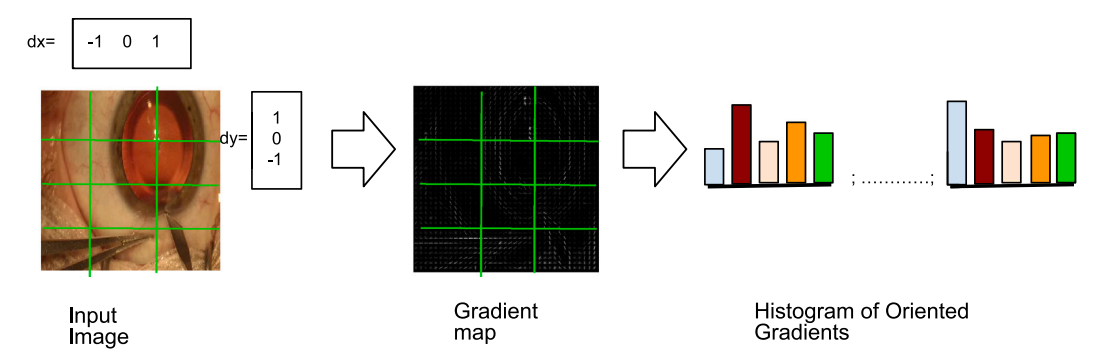
\includegraphics[width=0.80\textwidth]{2/figures/HOG.png}
                \caption{Proceso de Histogram of Oriented Gradients (HOG). Fuente:\cite {bhattarai2023hog}.}

                \label{1:fig}
            \end{figure}
            

        \end{itemize} 
\end{itemize}


\subsection{Deep Learning}
El Deep Learning ha transformado el campo del procesamiento de imágenes al permitir la automatización de tareas complejas como la clasificación, detección de objetos y segmentación de imágenes. Las redes neuronales profundas, particularmente las redes neuronales convolucionales (CNNs), son la arquitectura principal utilizada para el análisis de imágenes debido a su capacidad para capturar características espaciales jerárquicas en los datos visuales.


\begin{figure}[H]
    \centering
    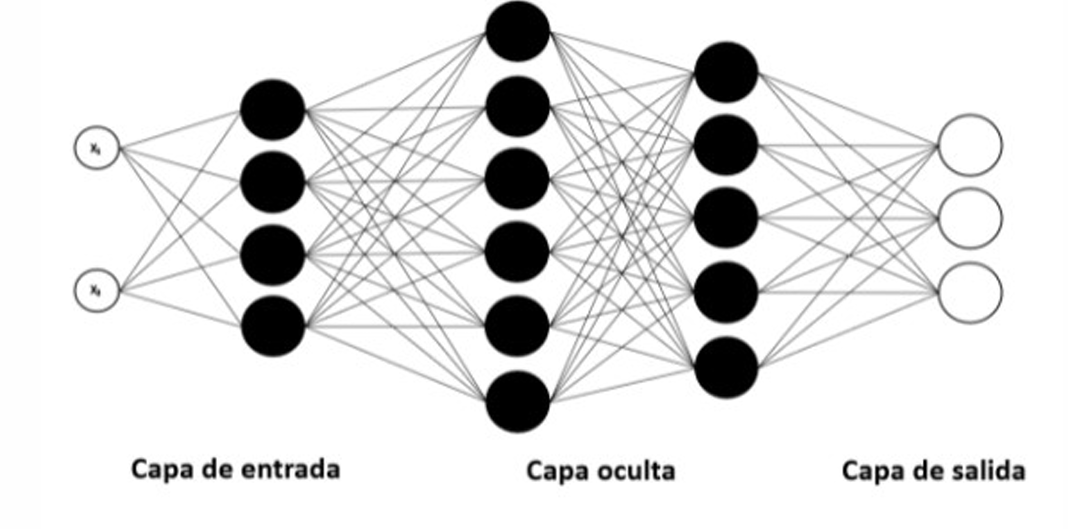
\includegraphics[width=0.60\textwidth]{2/figures/Redes neuronales.png}
    \caption{Estructura de una red neuronal. Fuente: Elaboración propia.}

\end{figure}

\subsubsection{Redes Neuronales Convolucionales (CNNs)}
Las Redes Neuronales Convolucionales (CNNs) constituyen una arquitectura clave dentro del Deep Learning, ampliamente reconocida por su eficacia en el análisis de imágenes. Su principal fortaleza radica en su capacidad para aprender representaciones jerárquicas de los datos visuales, lo que les permite captar patrones espaciales complejos. Las CNNs logran esta tarea mediante el uso de múltiples capas especializadas que procesan la información de manera progresiva.

Cada una de estas capas realiza la extracción automática de características relevantes de las imágenes, optimizando su capacidad de detección y clasificación durante el proceso de entrenamiento. Esta estructura en capas permite que las CNNs identifiquen desde bordes simples hasta patrones más abstractos, a medida que la información fluye desde las capas iniciales hacia las más profundas del modelo.

\begin{itemize} 
    \item 
    \textbf{Capa convolucional}: Esta capa aplica filtros (o kernels) sobre la imagen para extraer características locales como bordes, texturas y patrones. A medida que cada filtro se desplaza sobre la imagen, se genera un mapa de características que destaca las particularidades locales. Para una imagen de entrada \(X\), el resultado de aplicar un filtro \(K\) es un mapa de características \(F\) dado por:

    \[
    F(i,j) = \sum_m \sum_n X(i+m,j+n) \cdot K(m,n),
    \]

    donde \(m\) y \(n\) son los índices de los elementos del filtro \(K\), y \(i, j\) son los índices de los píxeles en la imagen.

    \begin{figure}[H]
        \centering
        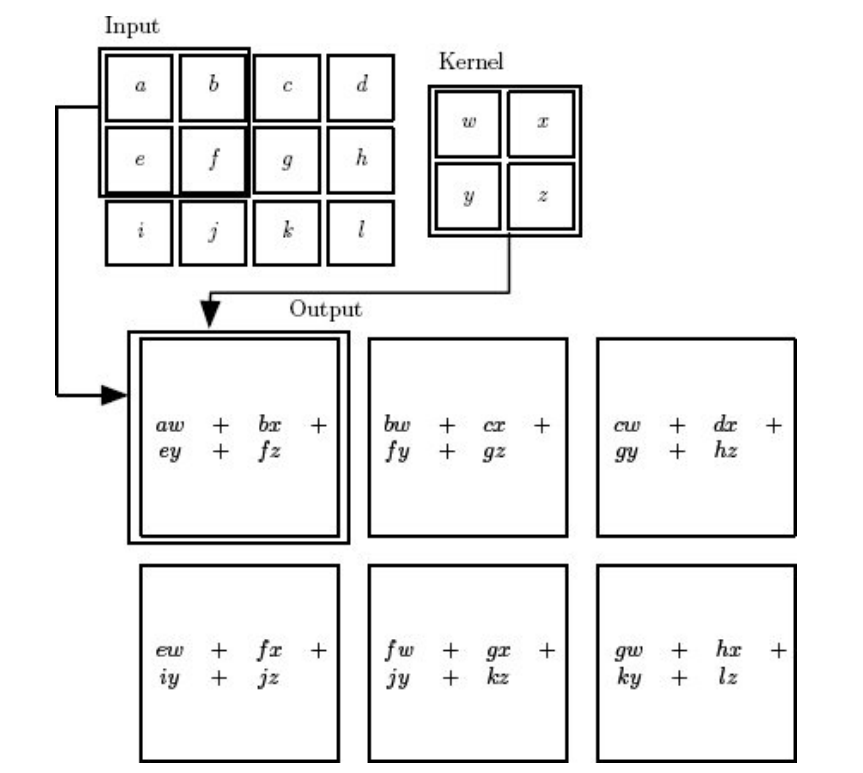
\includegraphics[width=0.40\textwidth]{2/figures/Convolucion.png}
        \caption{Proceso de convolución. Fuente: \cite{Goodfellow-et-al-2016}. \textit{Recuperado de Deep Learning}.}
        \label{fig:convolucion}
    \end{figure}
    

    \item \textbf{Capa de pooling}: Reduce la dimensionalidad de las características extraídas al resumir pequeñas regiones de las imágenes (por ejemplo, mediante el \textit{max-pooling}, que selecciona el valor máximo en cada región). Esto ayuda a reducir el número de parámetros y a controlar el sobreajuste.
\end{itemize}

\subsubsection{ResNet50}

La \textbf{ResNet50} es una arquitectura de red neuronal profunda que pertenece a la familia de las Redes Residuales (ResNet), introducida por He et al. en 2015. ResNet50 destaca por su capacidad para entrenar redes profundas sin enfrentar los problemas de degradación que afectan a las redes convolucionales tradicionales al aumentar en capas. Esto se logra mediante la incorporación de \textit{bloques residuales}, los cuales permiten una mejor propagación del gradiente a lo largo de las capas.

\paragraph{Arquitectura y Estructura de ResNet50}

ResNet50 está compuesta por 50 capas que incluyen convoluciones, \textit{pooling}, y capas totalmente conectadas. La clave de su arquitectura son los \textit{bloques residuales}, en los que la salida de una capa se suma directamente a la salida de una capa posterior, permitiendo que los datos "salten" una o más capas. Esta operación de "salto" ayuda a conservar la información y a mitigar la pérdida del gradiente, un problema común en redes profundas. La estructura de ResNet50 puede dividirse en:
\begin{itemize}
    \item \textbf{Bloques residuales}: Cada bloque consiste en una serie de capas convolucionales, seguidas de una conexión residual que permite sumar la entrada del bloque a la salida de una capa más profunda, facilitando el flujo de información.
    \item \textbf{Capas convolucionales y pooling}: La red comienza con una capa convolucional inicial y una operación de pooling, seguidas de los bloques residuales. Al final de la red, se realiza un \textit{global average pooling} para reducir la dimensionalidad antes de la capa totalmente conectada.
\end{itemize}

\paragraph{Funcionamiento de los bloques residuales}
Los bloques residuales son el componente esencial que diferencia a ResNet50 de otras arquitecturas. En cada bloque, una entrada \( x \) se combina con la salida de una convolución \( F(x) \) mediante una suma: 
\[
y = F(x) + x,
\]
donde \( F(x) \) es la salida de las capas convolucionales del bloque. Esta suma permite que el bloque aprenda la función de residuo en lugar de una transformación completa, lo que facilita el entrenamiento y previene el desvanecimiento del gradiente.

\paragraph{Ventajas de ResNet50}
ResNet50 es ampliamente utilizada como extractor de características en tareas de visión por computadora debido a su capacidad para aprender y representar características visuales complejas. Sus principales ventajas como extractor de características incluyen:

\begin{itemize}
    \item \textbf{Profundidad eficaz}: La arquitectura profunda de ResNet50, soportada por bloques residuales, permite extraer características de alta calidad y precisión sin sufrir degradación de rendimiento, lo que resulta en descriptores visuales detallados y robustos.
    \item \textbf{Capacidad de transferencia de aprendizaje}: Al estar preentrenada en grandes conjuntos de datos como ImageNet, ResNet50 ofrece una base de características generalizables, permitiendo su uso en diversas aplicaciones de extracción de características sin necesidad de entrenar el modelo desde cero.
    \item \textbf{Optimización computacional}: La eficiencia en el flujo de gradientes gracias a los bloques residuales mejora la velocidad de extracción y permite el uso de ResNet50 en múltiples plataformas, facilitando un procesamiento eficiente incluso en sistemas con limitaciones de hardware.
\end{itemize}

\begin{figure}[H]
	\centering
	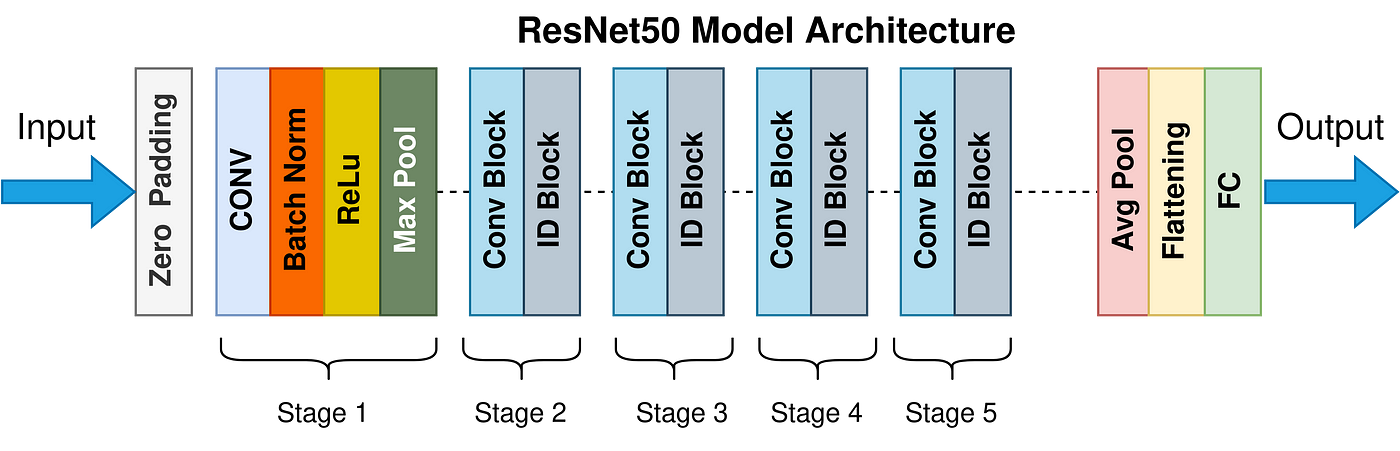
\includegraphics[width=0.80\textwidth]{2/figures/ResNet.png}
	\caption{Arquitectura de ResNet50. Fuente:\cite {Mukherjee2022}.}

	\label{1:fig}
\end{figure}

\subsection{Análisis de Componentes Principales (PCA)}

El \textbf{Análisis de componentes principales} (PCA, por sus siglas en inglés) es una técnica estadística utilizada para la \textit{reducción de dimensionalidad} en conjuntos de datos de alta dimensión. PCA transforma los datos en un espacio de menor dimensión mientras conserva la mayor variabilidad posible, lo cual es útil en el preprocesamiento de datos para reducir la redundancia y simplificar el análisis.

\subsubsection{Funcionamiento de PCA}

El proceso de PCA se basa en los siguientes pasos:

\begin{enumerate}
    \item \textbf{Centramiento de los datos}: 
    Dado un conjunto de datos con \(n\) muestras y \(d\) características, se calcula la media de cada característica y se centra cada variable restando su media. Esto garantiza que el nuevo conjunto de datos tenga una media de cero, simplificando los cálculos subsiguientes. Si \(\mathbf{X}\) representa la matriz de datos original, donde cada columna es una característica, la matriz centrada \(\mathbf{X_c}\) se obtiene restando la media:
    
    \[
    \mathbf{X_c} = \mathbf{X} - \text{mean}(\mathbf{X})
    \]

    \item \textbf{Cálculo de la matriz de covarianza}: 
    La matriz de covarianza \(\mathbf{C}\) representa cómo cada par de variables varía conjuntamente, permitiendo identificar relaciones entre las características originales. La matriz de covarianza se calcula como:

    \[
    \mathbf{C} = \frac{1}{n-1} \mathbf{X_c}^T \mathbf{X_c}
    \]

    donde \(n\) es el número de muestras en el conjunto de datos. Esta matriz es de tamaño \(d \times d\), donde \(d\) es el número de características.

    \item \textbf{Descomposición de la matriz de covarianza en valores y vectores propios}: 
    La descomposición de la matriz de covarianza permite encontrar los \textit{componentes principales}. Se calculan los \textit{vectores propios} y \textit{valores propios} de la matriz de covarianza \(\mathbf{C}\):

    \[
    \mathbf{C} \mathbf{v}_i = \lambda_i \mathbf{v}_i
    \]

    donde \(\mathbf{v}_i\) es el vector propio (o componente principal) y \(\lambda_i\) es su valor propio correspondiente, que representa la varianza explicada por ese componente. Los componentes se ordenan en función de la magnitud de \(\lambda_i\), de mayor a menor, ya que los valores propios más altos representan mayor variabilidad en los datos.

    \item \textbf{Selección de componentes principales}: 
    A menudo, se seleccionan solo los primeros \(k\) componentes principales que explican la mayor parte de la varianza de los datos. La cantidad de varianza explicada por cada componente principal se calcula como:

    \[
    \text{Varianza Explicada} = \frac{\lambda_i}{\sum_{j=1}^{d} \lambda_j}
    \]

    y se suele visualizar en un gráfico de varianza explicada acumulada para elegir un valor óptimo de \(k\). El método del codo también es común para identificar el número de componentes principales.

    \item \textbf{Proyección de los datos en el espacio reducido}: 
    Finalmente, los datos originales se proyectan sobre los \(k\) componentes seleccionados para obtener una representación de menor dimensión. Sea \(\mathbf{V}_k\) la matriz de componentes principales seleccionados (de tamaño \(d \times k\)), entonces la matriz de datos proyectada \(\mathbf{X_p}\) en el espacio reducido es:

    \[
    \mathbf{X_p} = \mathbf{X_c} \mathbf{V}_k
    \]

    donde \(\mathbf{X_p}\) es la versión reducida de los datos, con \(k\) dimensiones en lugar de \(d\), pero manteniendo la mayor parte de la información original.
\end{enumerate}

\subsubsection{Ventajas de PCA}

PCA ofrece varias ventajas importantes en el análisis de datos:

\begin{itemize}
    \item \textbf{Reducción de dimensionalidad}: Al transformar los datos a un espacio de menor dimensión, PCA facilita el análisis y visualización de datos de alta dimensionalidad.
    \item \textbf{Eliminación de redundancia}: Al seleccionar los componentes principales que explican la mayor parte de la varianza, PCA reduce las dimensiones y elimina las variables redundantes.
    \item \textbf{Optimización del rendimiento}: Al reducir el número de dimensiones, PCA disminuye la complejidad computacional, optimizando el rendimiento de algoritmos de machine learning que usan los datos proyectados.
\end{itemize}



\subsection{Clustering}
Es una técnica de aprendizaje no supervisado que agrupa un conjunto de datos en subconjuntos llamados \textit{clusters}, de manera que los objetos dentro de un mismo cluster sean más similares entre sí que con los de otros clusters. Es una herramienta clave en la minería de datos, el análisis de datos y el aprendizaje automático.

A diferencia del aprendizaje supervisado, donde se dispone de etiquetas de clase, el clustering busca encontrar estructuras ocultas en los datos sin conocimiento previo de las etiquetas.

\subsubsection{K-means}
Su objetivo es dividir un conjunto de datos en \(k\) grupos o \textit{clusters}, minimizando la varianza dentro de cada grupo. La esencia de K-means es encontrar \(k\) centroides, uno para cada cluster, de manera que los puntos de datos dentro de un cluster estén más cerca de su propio centroide que de cualquier otro.

Dado un conjunto de datos \(X = \{x_1, x_2, \dots, x_n\}\) donde cada \(x_i \in \mathbb{R}^d\), el algoritmo K-means intenta particionar los datos en \(k\) clusters \(C = \{C_1, C_2, \dots, C_k\}\), tal que se minimice el criterio de suma de los cuadrados de las distancias (SSE, \textit{Sum of Squared Errors}) entre los puntos y sus respectivos centroides.

La función objetivo que el algoritmo K-means intenta minimizar es la siguiente:

\[
J(C) = \sum_{i=1}^{k} \sum_{x_j \in C_i} \| x_j - \mu_i \|^2,
\]

donde:
\begin{itemize}
    \item \(C_i\) es el \(i\)-ésimo cluster,
    \item \(\mu_i = \frac{1}{|C_i|} \sum_{x_j \in C_i} x_j\) es el centroide del cluster \(C_i\), calculado como el promedio de los puntos de datos asignados a ese cluster,
    \item \(\| x_j - \mu_i \|\) es la distancia Euclidiana entre un punto \(x_j\) y el centroide \(\mu_i\).
\end{itemize}

Esta función mide la compacidad de los clusters. El objetivo del algoritmo es minimizar \(J(C)\), es decir, minimizar la suma de las distancias al cuadrado entre los puntos de datos y sus centroides correspondientes.

\begin{figure}[H]
    \centering
    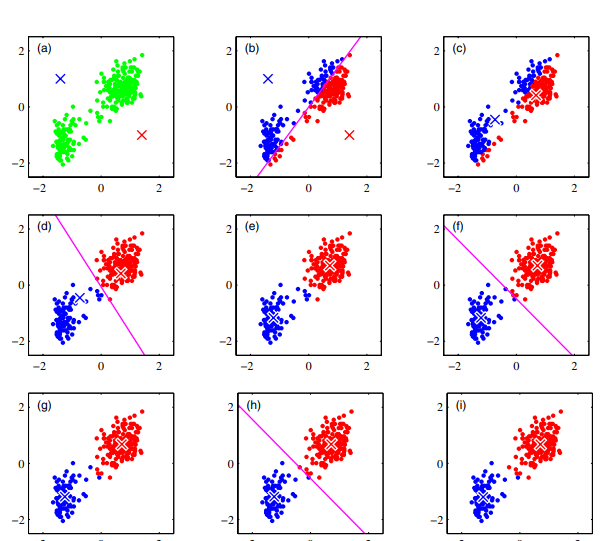
\includegraphics[width=0.40\textwidth]{2/figures/Kmeans.png}
    \caption{Ilustración de K-means. Fuente: \cite{bishop2006pattern}. \textit{Recuperado de Pattern Recognition and Machine Learning}.}
    \label{fig:kmeans}
\end{figure}


\subsection{Inercia en clustering}

En el análisis de clustering, la \textbf{inercia} es una medida de la dispersión interna de los datos dentro de un conjunto de clusters. En términos prácticos, la inercia cuantifica cuán estrechamente agrupados están los puntos de datos alrededor de los centroides de sus respectivos clusters. Esta medida es particularmente relevante en el algoritmo de \textit{K-means}, donde se busca minimizar la inercia para asegurar que cada cluster esté lo más compacto posible.

\subsubsection{Definición de inercia}

La inercia, también conocida como \textit{within-cluster sum of squares} (WCSS), se calcula como la suma de las distancias cuadradas entre cada punto de datos y el centroide de su cluster asignado. Matemáticamente, si tenemos un conjunto de datos \(X = \{x_1, x_2, \dots, x_n\}\) agrupado en \(k\) clusters \(C = \{C_1, C_2, \dots, C_k\}\), la inercia se define como:

\[
\text{Inercia} = \sum_{i=1}^{k} \sum_{x_j \in C_i} \| x_j - \mu_i \|^2
\]

donde:
\begin{itemize}
    \item \(C_i\) es el \(i\)-ésimo cluster,
    \item \(x_j\) representa cada punto de datos perteneciente al cluster \(C_i\),
    \item \(\mu_i\) es el centroide del cluster \(C_i\), calculado como el promedio de los puntos de datos dentro de \(C_i\),
    \item \(\| x_j - \mu_i \|\) es la distancia euclidiana entre el punto \(x_j\) y el centroide \(\mu_i\).
\end{itemize}

La inercia mide, por tanto, la compactación de los clusters: a menor inercia, mayor cohesión interna en cada cluster.

\subsubsection{Optimización de clusters mediante inercia}

La minimización de la inercia es uno de los objetivos principales en el algoritmo \textit{K-means}, ya que un valor bajo de inercia indica que los puntos de datos están más cerca de sus centroides, lo cual sugiere que los clusters son compactos y bien definidos. Sin embargo, la inercia tiende a disminuir a medida que se incrementa el número de clusters, lo que puede llevar a una sobreajuste si no se controla.

\subsubsection{Método del codo}

El \textbf{método del codo} es una técnica gráfica que utiliza la inercia para determinar el número óptimo de clusters en un conjunto de datos. Este método consiste en calcular la inercia para diferentes valores de \(k\) (número de clusters) y representar la inercia en función de \(k\). A medida que se aumenta \(k\), la inercia disminuye, ya que los clusters se vuelven más pequeños y específicos. Sin embargo, a partir de cierto punto, el beneficio de añadir clusters adicionales se reduce y la curva de inercia comienza a estabilizarse, formando un “codo”.

El punto donde se forma este “codo” en la gráfica indica el número de clusters óptimo. Elegir el valor de \(k\) en el codo permite obtener una buena estructura de clusters sin introducir clusters adicionales que solo disminuyan marginalmente la inercia.

\subsubsection{Ventajas de la Inercia}

La inercia ofrece una serie de beneficios al evaluar la calidad de los clusters:
\begin{itemize}
    \item \textbf{Cohesión de los clusters}: Minimizar la inercia asegura que los puntos dentro de cada cluster estén lo más cerca posible de sus centroides, lo que implica una alta cohesión interna.
    \item \textbf{Facilidad de interpretación}: La inercia es una medida intuitiva y directa para evaluar la dispersión de los datos, proporcionando una métrica clara para comparar diferentes agrupamientos.
    \item \textbf{Aplicabilidad en el Método del Codo}: La inercia es fundamental en el método del codo, que permite identificar de manera gráfica el número de clusters óptimo, optimizando así la estructura del agrupamiento.
\end{itemize}

